\chapter{Theoretical Background}
\label{chap:theoretical-background}

\section{Natural Language Processing}
Natural Language Processing is the field of Artificial Intelligence that gives the computers ability to understand text and spoken words in the same way human beings can. Natural Language Processing is a very broad field, it includes many sub-fields, such as text classification, name entity recognition, machine translation, etc. In this thesis, we focus on text classification and name entity recognition.

\section{Intent Classification}

Intent classification is the text classification task that aims to classify the user's input into a predefined set of intents. For example, in the case of a rental house search, the user's input "I want to rent a house in Ho Chi Minh City" is classified into the "rent\_house" intent.

There are two main approaches to intent classification: rule-based and machine learning-based. The rule-based approach uses a set of rules to classify the user's input. For example, the rule "if the user's input contains the word 'rent' and the word 'house', then the intent for this sentence is 'rent\_house'". One major drawback of the rule-based approach is that it requires a lot of effort and domain knowledge to create these rules.


The machine learning-based approach uses machine learning algorithms to learn the mapping between the user's input and the intent. Intent classification is a supervised learning problem, so the machine learning algorithm needs to be trained on the dataset of the user's input and the corresponding intent. The machine learning-based approach is more flexible than the rule-based approach because it does not require domain knowledge to create the rules. However, it requires a large amount of data to train the machine learning algorithm.

\section{Name Entity Recognition (NER)}
Name Entity Recognition is the task that determines the entities in the user's input. Figure \ref{fig:ner_example} illustrates an example of NER. In this example, we have 3 entities: "Sebastian Thrun" (Person), "Google" (Organization), and "2007" (Date).

\begin{figure}[ht]
    \centering
    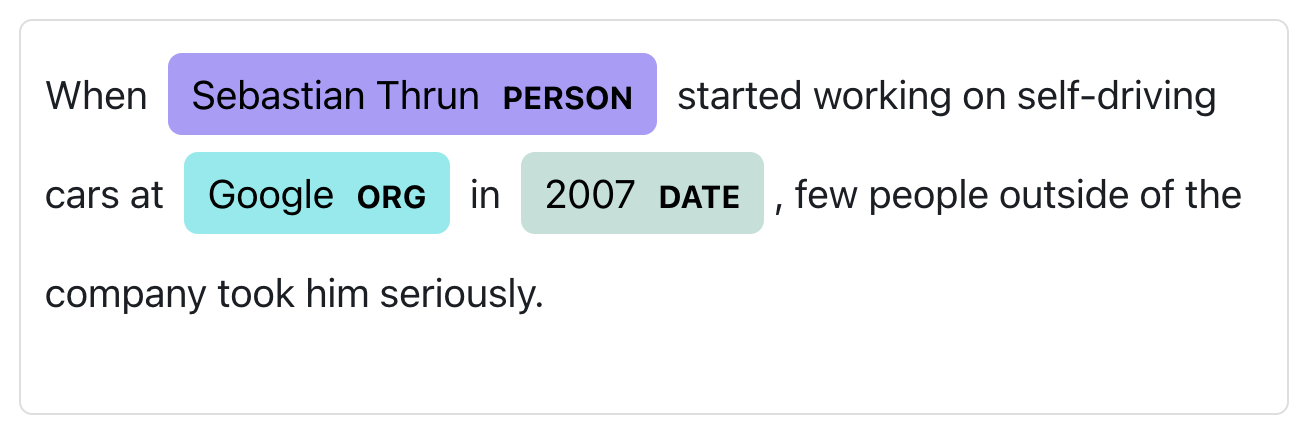
\includegraphics[width=0.8\textwidth]{Images/5.Theoretical_Background/ner_example.png}
    \caption{Example of NER, from \cite{spacy-visualizer-doc}}
    \label{fig:ner_example}
\end{figure}


To train the model for NER, we need to annotate the entities in the dataset. The popular format for annotating is BIO. In the BIO annotation, each word in the user's input is annotated with one of three labels: B, I, or O. The B label indicates the beginning of an entity, the I label indicates the inside of an entity, and the O label indicates that the word is not an entity. For example, the user's input "I want to rent a house in Ho Chi Minh City." is annotated as follows (Table \ref{tab:bio_annotation})

\begin{table}[ht]
    \centering
    \begin{tabular}{|c|c|c|c|c|c|c|c|c|c|c|}
        \hline
        I & want & to & rent & a & house & in & Ho & Chi & Minh & city \\    
        \hline
        O & O    & O  & B-TRAN & O & B-TYPE & O  & B-LOC    & I-LOC & I-LOC & I-LOC \\
        \hline
    \end{tabular}
    \caption{Example of BIO annotation}
    \label{tab:bio_annotation}
\end{table}

\section{Language Model}
A language model is a model that can determine the probability of the sequences of words. A language model is trained on a large dataset of text to predict the next word in the given context. The training process aims to enable the model to learn the patterns, structures, and relationships present in that language. 

There are two main types of language models: statistical-based models and neural network-based models. One of the most popular pure statistical language models is the n-grams model. These models are based on the consumption that the probability of the next word depends only on the previous n-1 words. However, these models have some drawbacks such as the inability to capture the long-term dependencies between the words. For that reason, the neural network language models are introduced and have become state-of-the-art in NLP. The neural network language models can understand complex patterns and capture the contextual information of the words.

\section{Word Representation}
Neural networks and deep learning can only take the numerical values as the input, so we need to convert the words into the numerical values. So in natural language processing, we need a way to represent the words as the numerical values. There are many techniques for word representation, such as One-hot representation, Bag of Words, TF-IDF, Word2Vec, etc. 

\subsection{One-hot representation}
To understand the one-hot representation, we need to understand the concept of vocabulary. The vocabulary is the set of all words in the corpus. For example, consider the corpus contains 2 sentences: "I want to rent a house in Ho Chi Minh City" and "I want to lease a room in District 1". The vocabulary of this corpus is \{"I", "want", "to", "rent", "a", "house", "in", "Ho", "Chi", "Minh", "city", "lease", "room", "district", "1"\}.

One-hot representation is the technique of converting the words into the one-hot vectors. The one-hot vector is the vector that has a length equal to the number of words in the vocabulary. The one-hot vector has a value of 1 at the index of the word in the vocabulary, and a value of 0 at the other indices. Consider the example vocabulary above, the one-hot vector of the word "rent" is [0, 0, 0, 1, 0, 0, 0, 0, 0, 0, 0, 0, 0, 0, 0]. Because the word "rent" is at the index 3 in the vocabulary, so the one-hot vector has the value of 1 at the index 3, and the value of 0 at the other indices.

\noindent The one-hot representation is very simple, but it has some drawbacks. 
\begin{itemize}
    \item The one-hot representation does not preserve the semantic relationships of the words. We want words that have similar meanings to also have similar representations.
    \item The one-hot representation is a sparse vector (the vector has only 1 non-zero value). The problem is that it requires a high-dimensional vector to represent the words, so training becomes slower and more complex. For example, we have 10000 words in the vocabulary, so we need a vector with a length of 10000 to represent each word.
\end{itemize}

\subsection{Word Embedding}
Word Embedding appears to solve the limitations of some traditional methods like one-hot encoding or Bag of Words. Word embedding is the technique that converts words into dense vectors in a low-dimensional vector space, preserving the semantic relationships of the words.

Figure \ref{fig:word_embedding} illustrates an example of Word Embedding representation in 2D space. In this example, the words in the same topics are close to each other. As a result, we have clusters for words in other topics, such as city, food, travel, etc. This example shows that Word Embedding can preserve the semantic meaning of the words.

\begin{figure}[ht]
    \centering
    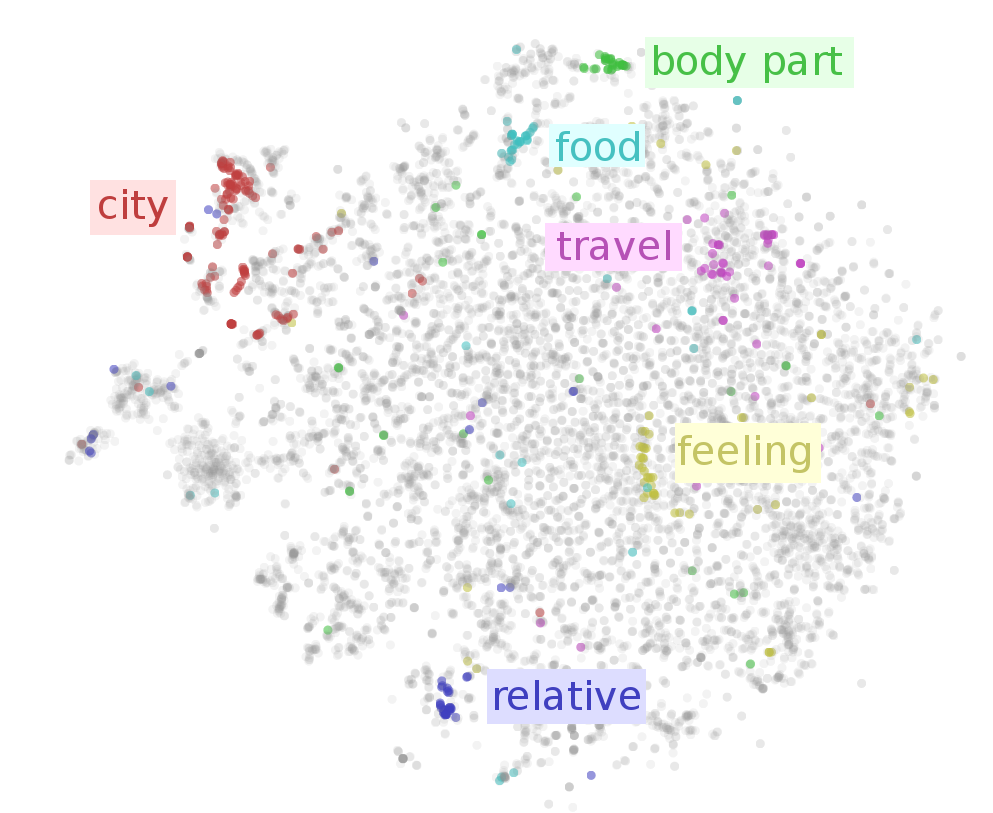
\includegraphics[width=0.3\textwidth]{Images/5.Theoretical_Background/word_embeddings_example.png}
    \caption{Example of Word Embedding representation in 2D space, From \cite{word-embedding-example}}
    \label{fig:word_embedding}
\end{figure}

There are some common word embedding models, such as Word2Vec, GloVe, FastText, etc. 

\subsection{Word2Vec}
Word2Vec is the popular word embedding technique. It was introduced by a team of researchers of Google, led by Tomas Mikolov in 2013 \cite{word2vec-paper-publication}. The key idea of Word2Vec is to learn word embedding by training a simple neural network. There are two main architectures for Word2Vec: Continuous Bag of Words (CBOW) and Skip-gram.
\begin{itemize}
    \item \textbf{Continuous Bag of Words (CBOW)}: The CBOW model predicts the current word based on the context. The CBOW architecture is similar to the feed-forward neural network, but it does not have the non-linear hidden layer to remove the computational complexity and the projection layer is shared for all words. The projection layer refers specifically to the layer responsible for transforming the input data (e.g., one-hot encoded vectors representing words) into a continuous vector space. The model architecture is shown in Figure \ref{fig:cbow_vs_skipgram}. 
    \item \textbf{Skip-gram}: The second architecture is similar to CBOW, but instead of predicting the current word based on the context, it tries to predict the surrounding words give the current word.
\end{itemize}

\begin{figure}[ht]
    \centering
    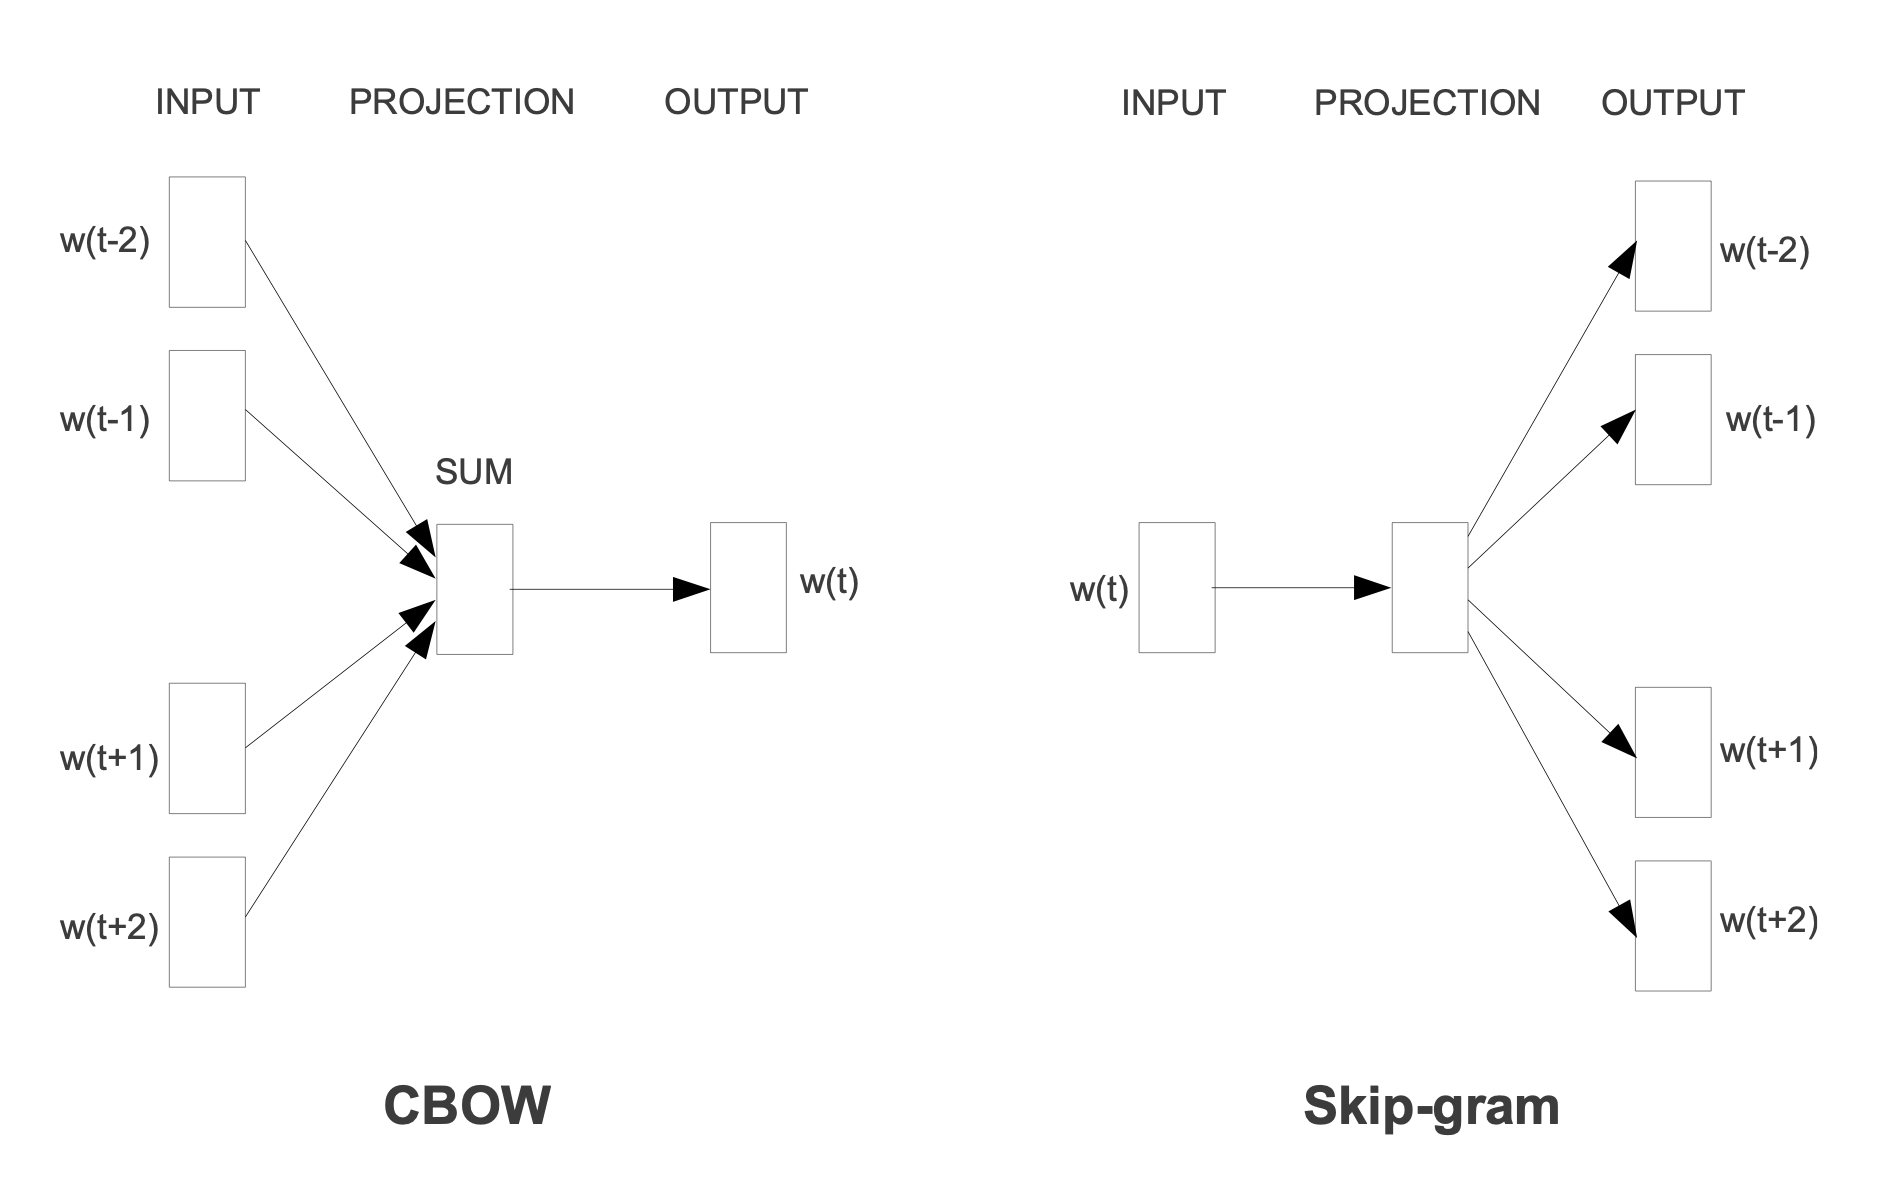
\includegraphics[width=0.8\textwidth]{Images/5.Theoretical_Background/cbow_vs_skipgram.png}
    \caption{The CBOW architecture predicts the current word based on the context, and the Skip-gram predicts surrounding words given the current word, From \cite{word2vec-paper-publication}}
    \label{fig:cbow_vs_skipgram}
\end{figure}

The training process involves backward propagation which adjusts the weights of the projection layer. The output of the projection layer is the word embedding that we want to get.

\subsection{Language Model for Word Embedding}
Although the pre-trained word embedding methods, such as Word2Vec, GloVe, FastText, etc can represent the word in the vector format, these are non-contextual word embedding. Because they can not capture the context of the words. For example, the word "Apple" has different meanings in the sentences "Apple releases the new MacbookPro" and "Apples are a good source of vitamin C". The word "Apple" in the first sentence refers to the technology company while the word "Apple" in the second sentence refers to the fruit. The traditional word embedding methods only represent the word "Apple" with one fixed vector, so it cannot distinguish these two meanings of the word "Apple".

The Language Model for Word Embedding technique uses the language model to create contextual word embeddings. Some popular Language Models for Word Embedding are ELMo, BERT, GPT, etc. These language models can capture the context of the words, due to the model architecture using some Sequence Neural Networks like ELMo or using transformer architecture like BERT. The architecture of these language models will be discussed in the next sections.

\section{Recurrent Neural Network (RNN)}
A Recurrent Neural Network (RNN) is a type of neural network model to deal with sequential data. Sequential data is data arranged in sequences such as text, speech, and time series, where the order of the data point is important. The RNN models allow the information to persist through the time steps, so it can capture the context of the words. For that reason, RNN models are widely used in the Natural Language Processing field.

\subsection{Architecture of FeedForward Neural Network}
Before going into the architecture of RNN models, we need to understand why the feedforward neural network models are limited in their ability to handle sequential data. Consider the feedforward neural network in Figure \ref{fig:feedforward_architecture}, the output $y_{i}$ only depends on the input layer, but there are some problems that the output $y_{i}$ also depend on the previous output $y_{j}$, $y_{j-1}$, $y_{j-2}$, etc. For example, in the Part-of-Speech tagging, if the model already has the two previous words as nouns and verbs respectively, then the current word is likely to be a noun. There are some relationships between the words in the sentence, but with the architecture, the feedforward neural network cannot capture these relationships.

\begin{figure}[ht]
    \centering
    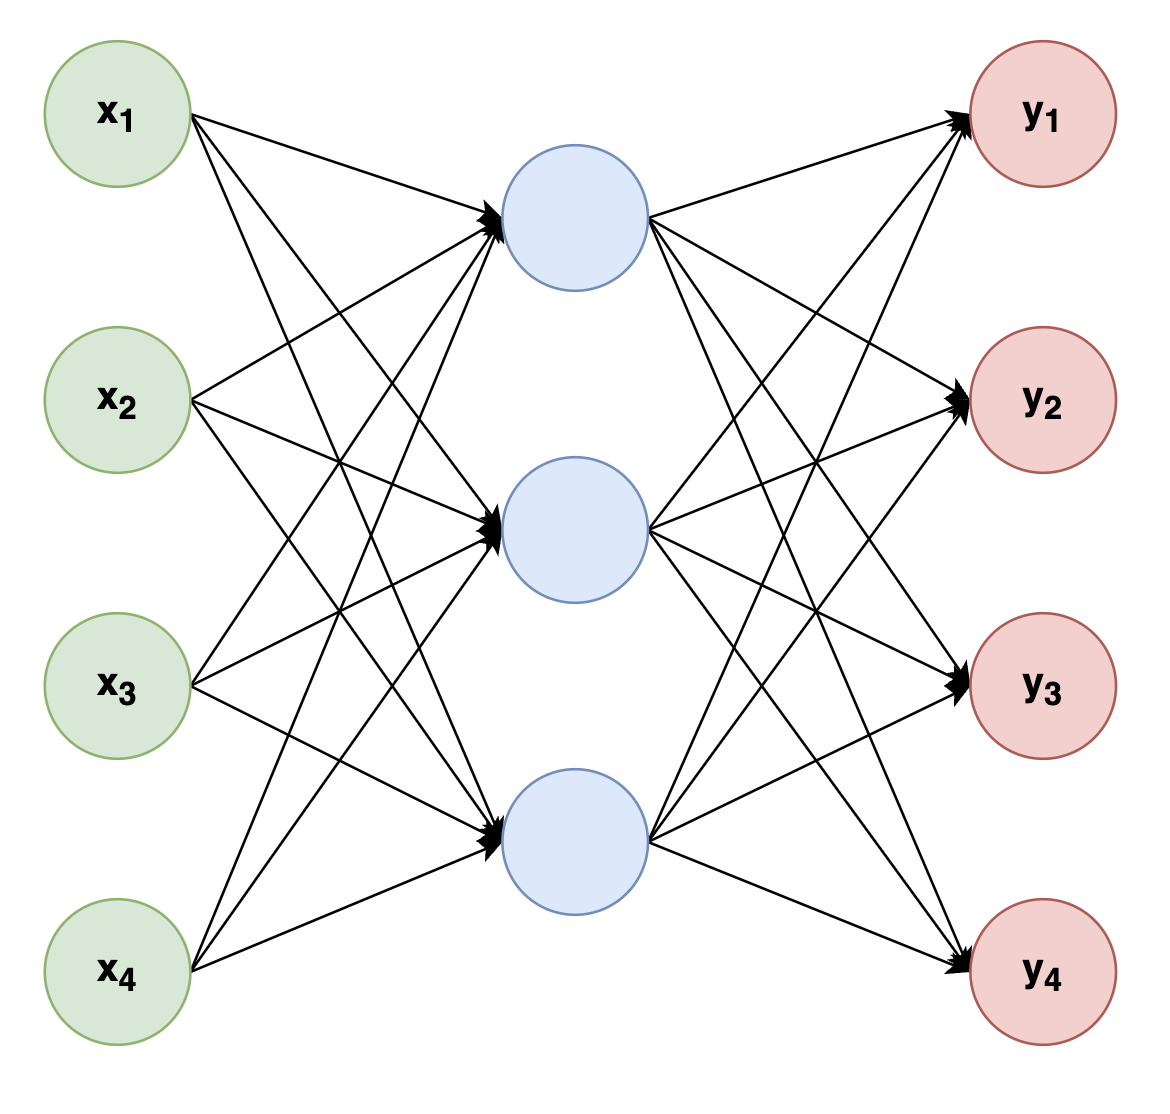
\includegraphics[width=0.4\textwidth]{Images/5.Theoretical_Background/feedforward_architecture.png}
    \caption{The architecture of feedforward neural network}
    \label{fig:feedforward_architecture}
\end{figure}

One major drawback of the feedforward neural network is that it only accepts the fixed-length input. However, the length of the sequential data is not fixed, so we need a model that can accept the variable-length input.

\subsection{Architecture of Recurrent Neural Network}
To solve the problem of feedforward neural networks, the Recurrent Neural Network (RNN) has a feedback loop that allows previous outputs to be used as inputs. The architecture of RNN is shown in Figure \ref{fig:rnn_fold} where the feedback loop is the red line. Another way to visualize the RNN architecture is to unfold the RNN into the sequence of the feedforward neural network as shown in Figure \ref{fig:rnn_unfold}

\begin{figure}[ht]
    \centering
    \begin{subfigure}[b]{0.3\textwidth}
        \centering
        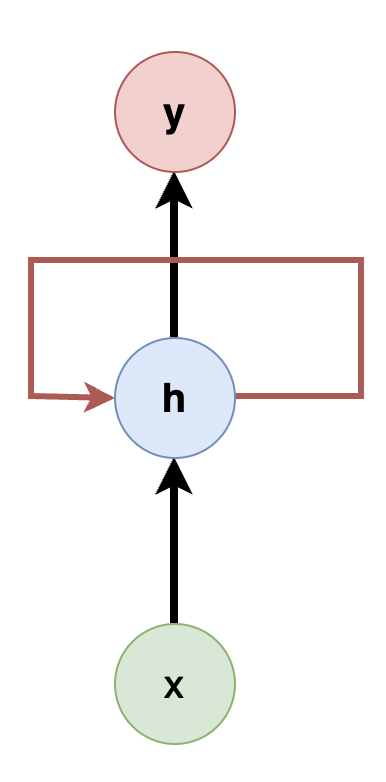
\includegraphics[height=0.25\textheight]{Images/5.Theoretical_Background/rnn_fold.png}
        \caption{RNN folded}
        \label{fig:rnn_fold}
    \end{subfigure}
    \begin{subfigure}[b]{0.65\textwidth}
        \centering
        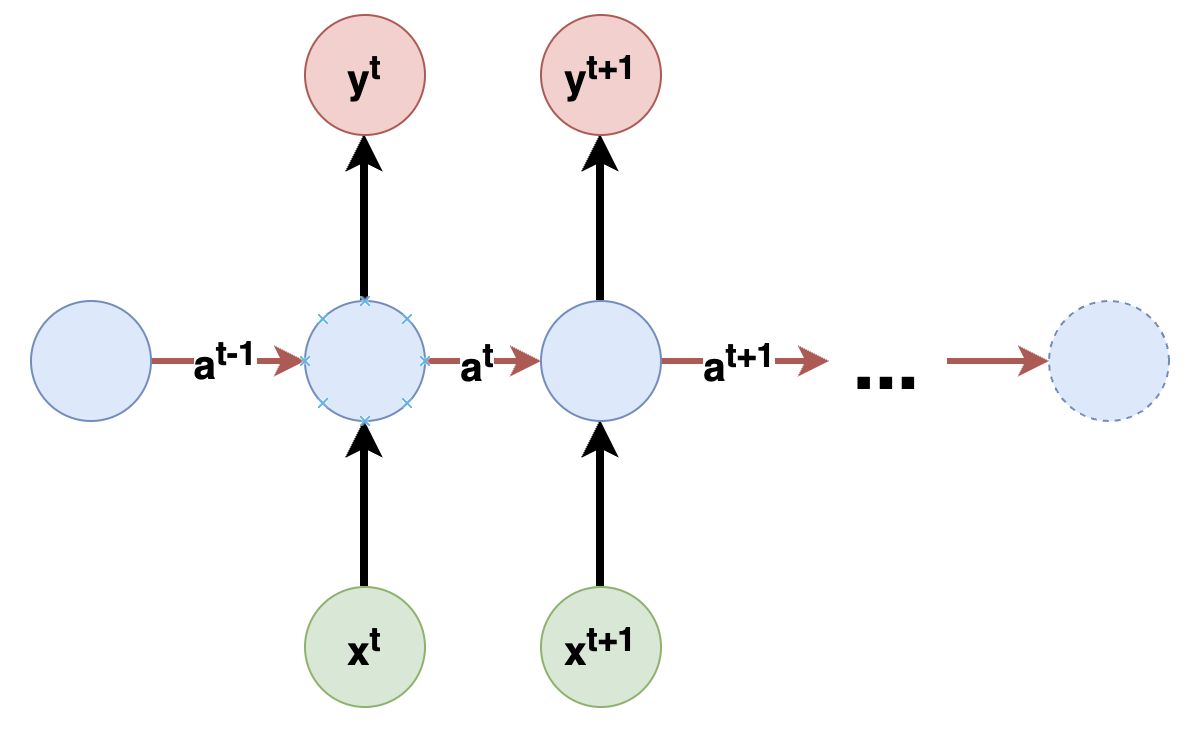
\includegraphics[height=0.25\textheight]{Images/5.Theoretical_Background/rnn_unfold.png}
        \caption{RNN unfolded}
        \label{fig:rnn_unfold}
    \end{subfigure}
    \caption{The architecture of RNN}
\end{figure}

The basic idea behind RNN is to use the hidden state $a^{<t-1>}$ from the previous time step as the input for the current step. The output $y^{<t>}$ and the hidden state $a^{<t>}$ is calculated as follows:

\begin{align*}
    a^{<t>} &= g_{1}(W_{aa}a^{<t-1>} + W_{ax}x^{<t>} + b_a) \\
    y^{<t>} &= g_{2}(W_{ya}a^{<t>} + b_y)
\end{align*}

\noindent where $g_{1}$ and $g_{2}$ are the activation functions, $W_{aa}$, $W_{ax}$, $W_{ya}$, are the weight matrices, $b_a$ and $b_y$ are the bias vectors. All of these parameters are the same over the time steps and are trained during the training process.

\subsection{The applications of RNN models}
There are many applications of RNN in the Natural Language Processing field such as text classification, name entity recognition, machine translation, etc. Based on the application, the RNN model can have different architectures. The RNN architectures and their applications are shown in Table \ref{tab:rnn_architecture}.

\begin{longtable}[ht]{| l | c | l |}
    \hline
    Type of RNN & Architecture & Application \\
    \hline
    One-to-Many & 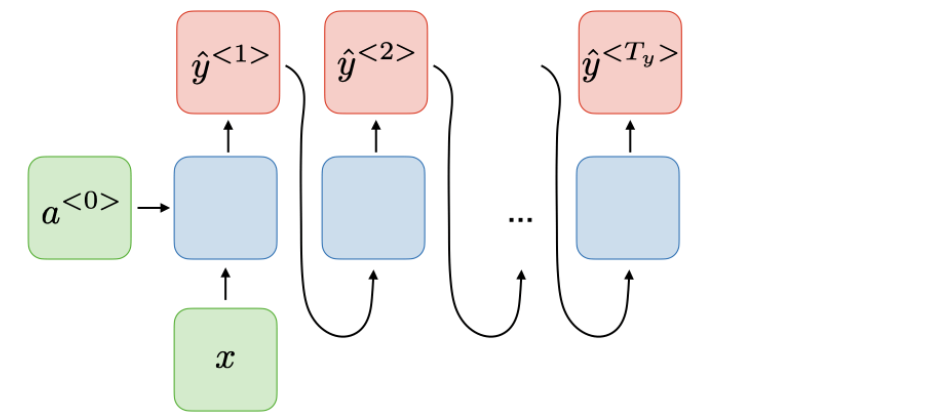
\includegraphics[width=0.5\textwidth]{Images/5.Theoretical_Background/rnn_one_to_many.png} & Text generation \\
    \hline
    Many-to-One & 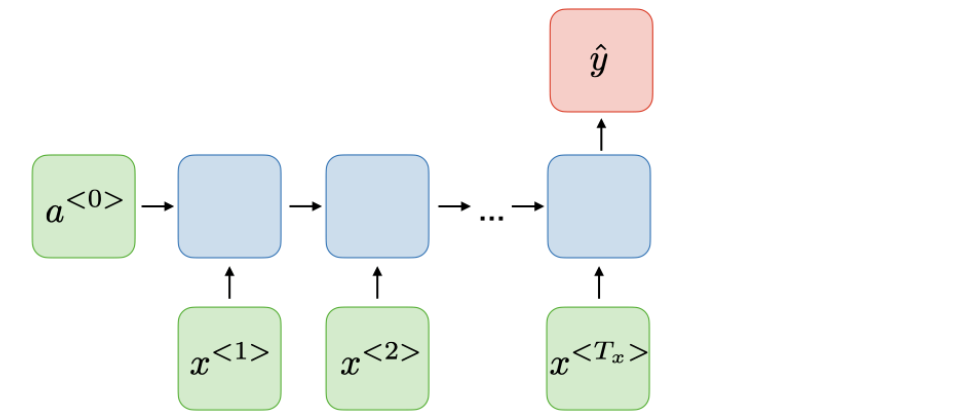
\includegraphics[width=0.5\textwidth]{Images/5.Theoretical_Background/rnn_many_to_one.png} & Text classification \\
    \hline
    Many-to-Many & 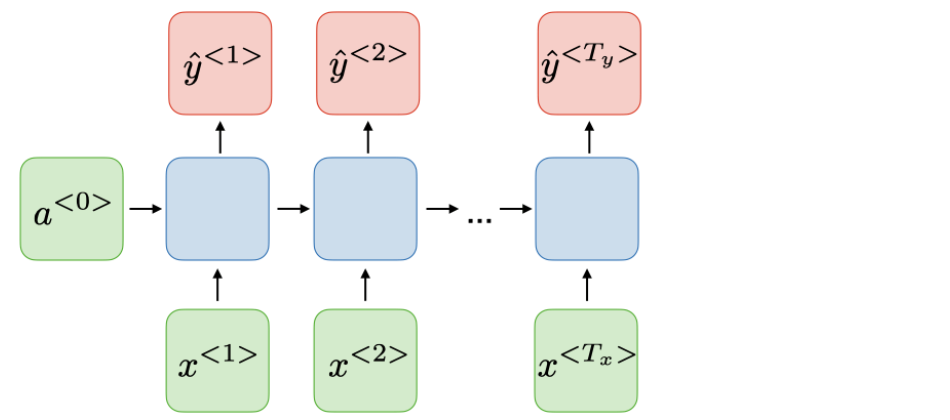
\includegraphics[width=0.5\textwidth]{Images/5.Theoretical_Background/rnn_many_to_many.png} & Name entity recognition \\
    \hline
    \caption{Different architectures of RNN}
    \label{tab:rnn_architecture}
\end{longtable}

\subsection{Disadvantages of RNN}
The training process of traditional RNN models consists of forward propagation (calculate the output from the beginning to the last time step) and backward propagation (calculate the gradients between the loss function and the parameters in the backward direction). Then these gradients are used to update the parameters. In the backward propagation process, the gradients can be very small or large. When the gradients are minimal, the parameters will not be updated, so the model fails to learn. It is called the vanishing gradient problem. Another problem is that the gradients can become exponentially large, so the model becomes very unstable and fails to optimize the weight matrix. It is called the exploding gradient problem. These problems make the training process of RNN models very difficult and unstable.

Besides, the information in RNN is propagated step by step from the first cell to the current cell, through each time step, the information is gradually lost, so the output of the RNN models mainly depends on the recent time steps. This leads to the problem that the RNN models cannot capture the long-term dependencies between the words.

\section{Long Short-Term Memory (LSTM)}
LSTM is a type of Recurrent Neural Network (RNN). The LSTM can deal with the vanishing gradient problem encountered by traditional RNNs. 

\subsection{LSTM architecture}
Consider the RNN cell and the LSTM cell in Figure \ref{fig:rnn_cell_vs_lstm_cell}. Similar to the RNN cell, the LSTM cell has the hidden state $a^{t}$. In addition to that, the LSTM also has a cell state represented by $c^{t-1}$ and $c^{t}$. The hidden state $a^{t}$ is used to capture the dependencies between the short-range time steps, so it is considered as the short-term memory. In contrast, the cell state $c^{t}$ could capture the dependencies between the long-range time steps, so it is considered as the long-term memory.

\begin{figure}[ht]
    \centering
    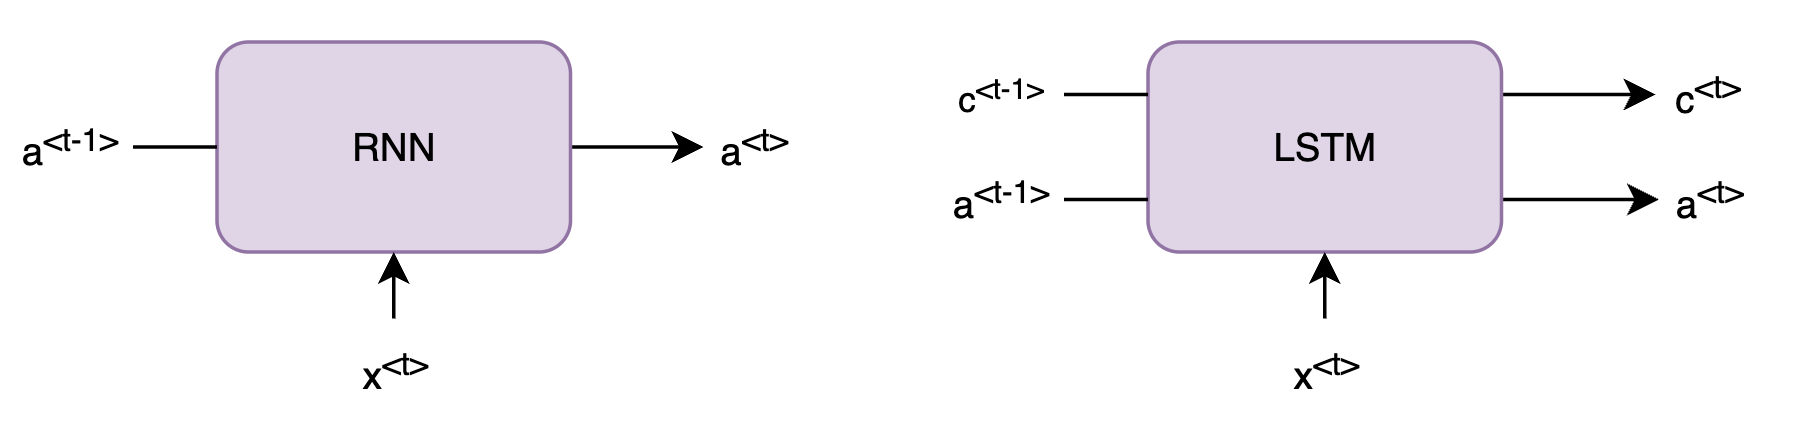
\includegraphics[width=0.7\textwidth]{Images/5.Theoretical_Background/rnn_vs_lstm_cell.png}
    \caption{The RNN cell and the LSTM cell}
    \label{fig:rnn_cell_vs_lstm_cell}
\end{figure}

The LSTM cell has 3 gates: the forget gate ($\Gamma_f$), the update gate($\Gamma_u$), and the output gate($\Gamma_o$). These gates control the flow of information through the cell. We have the following equations to calculate the gates and the cell state $c^{t}$:

\begin{align}
    \Gamma_f &= \sigma(W_f[a^{t-1}, x^{t}] + b_f) \\
    \Gamma_u &= \sigma(W_u[a^{t-1}, x^{t}] + b_u) \\
    \Gamma_o &= \sigma(W_o[a^{t-1}, x^{t}] + b_o) \\
    \tilde{c}^{t} &= tanh(W_c[a^{t-1}, x^{t}] + b_c) \label{eq:calcuate_c_tilde} \\
    c^{t} &= \Gamma_f * c^{t-1} + \Gamma_u * \tilde{c}^{t} \label{eq:calculate_c}\\
    a^{t} &= \Gamma_o * tanh(c^{t})
\end{align}

Based on the 3 first equations, we know that all the gates in the LSTM cell are calculated based on the previous hidden state $a^{t-1}$ and the current input $x^{t}$. The value of these three gates is between 0 and 1. In each cell, we have $\tilde{c}^{t}$ which is the candidate for the cell state $c^{t}$, representing the information in that cell. In equation \ref{eq:calculate_c}, the forget gate $\Gamma_f$ and the update gate $\Gamma_u$ decide which information to keep and which information to throw away. When the forget gate is nearly zero, it means the information $\tilde{c}^t$ in this cell is important and needs to be kept for the long term. In contrast, if the update gate is nearly zero, it means the information $\tilde{c}^t$ in this cell is not important and needs to be thrown away. So the $c^{t-1}$ is passed to the next cell. 

To sum up, the LSTM model can decide which information to keep and which information to throw away throughout the time steps. This allows the LSTM model to capture the important information for the long term and avoid the vanishing gradient problem.

\subsection{Bidirectional LSTM (BiLSTM)}
In some real scenarios, especially in the Natural Language Processing field, we need to get information from both the past and the future. It means that we need to consider the sequential data from both left to right and right to left directions. For example, two sentences: "Apple releases the new iPhone 12" and "Apple is a good source of vitamin C". With the traditional RNN models or the LSTM models, we only consider the context on the left of the words. So with these models, we can not distinguish the two meanings of the word "Apple". So we need a model that can capture the context of both sides of the word. That is the BiLSTM model.

The BiLSTM model consists of two LSTM layers, one layer processes the input sequence from the beginning to the end, and the other layer processes the input sequence from the end to the beginning. The output of the BiLSTM model is the concatenation of the outputs of the two LSTM layers. With this architecture, the BiLSTM model can capture the context of the previous words and the next words, so it is widely used in the Natural Language Processing field. The architecture of the BiLSTM model is shown in Figure \ref{fig:bilstm_architecture}.

\begin{figure}[ht]
    \centering
    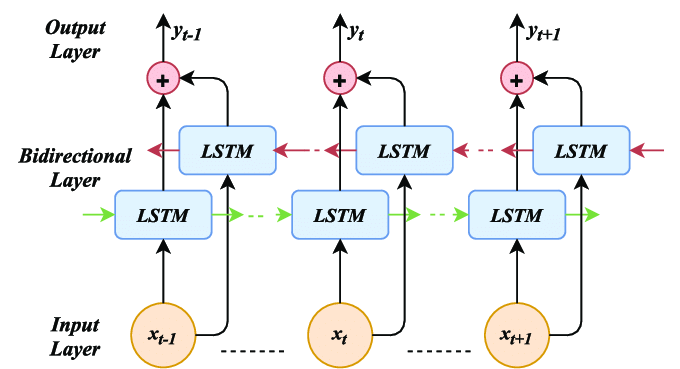
\includegraphics[width=0.8\textwidth]{Images/5.Theoretical_Background/bilstm_architecture.png}
    \caption{The architecture of the BiLSTM model, Source \cite{bilstm_medium} }
    \label{fig:bilstm_architecture}
\end{figure}

\section{Sequence to Sequence (Seq2Seq) Model}
The Sequence to Sequence model is a type of RNN model that takes a sequence of data (words, letters, time series data) as input and outputs another sequence of data. This model is applied to solve Natural Language Problems like machine translation, text summarization, question answering, etc...

There are two main components in the Seq2Seq model: the encoder and the decoder. Both the encoder and decoder are RNN models, usually LSTM models. The encoder takes the input sequence and encodes it into vectors (in the case of LSTM, these are the last hidden state and the cell state). The decoder takes these vectors from the encoder and decodes them into the output sequence. The architecture of the Seq2Seq model is shown in Figure \ref{fig:seq2seq_architecture}

\begin{figure}[ht]
    \centering
    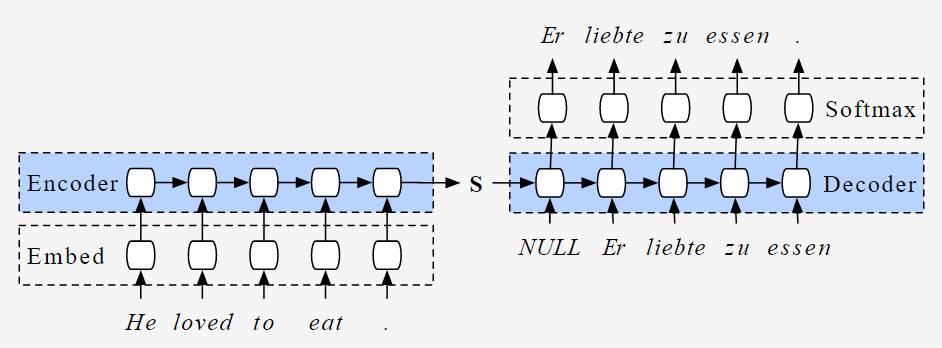
\includegraphics[width=0.8\textwidth]{Images/5.Theoretical_Background/seq2seq_architecture.png}
    \caption{Overall architecture of the Seq2Seq model, Source \cite{seq2seq_analyticsvidhya}}
    \label{fig:seq2seq_architecture}
\end{figure}

A problem with the original Seq2Seq model is that a neural network needs to compress all information of the input sequence into a fixed-length vector. This makes the model difficult to learn and deal with the long sentences. \cite{bahdanau2016neural}. The attention mechanism is the extension of the encoder-decoder architecture that solves this problem. Instead of encoding the whole input sentence, the attention mechanism allows the decoder to focus on the relevant parts of the input sentence when decoding each word. The attention mechanism is introduced in the next section.

\section{Attention}
In Psychology, attention is the human ability to selectively concentrate on one or a few things and ignore others. The Attention mechanism in NLP proposed in 2015 by Bahdanau et al in \cite{bahdanau2016neural} was inspired by this human ability. The key idea of the attention mechanism is at each time step, the decoder decides which part of the input sequence to focus on. To understand the attention mechanism, we consider the machine translation task.

We have the input sentence $x_1, x_2, x_3, ..., x_m$ in language A, and translation can be thought of as finding the output sentence $y_1, y_2, y_3, ..., y_n$ in language B. We use the encoder-decoder with an attention mechanism similar to Figure \ref{fig:attention_architecture} to solve this problem. The first step is that the encoder maps the input sentence $x_1, x_2, x_3, ..., x_m$ to a sequence of hidden states $s_1, s_2, s_3, ..., s_m$. Given the hidden states s, in each decoder time step, this model calculates the attention score between the decoder state $h_t$ and the encoder state $s_k$. The attention score shows how relevant is the source token k for target step t. Then it computes the attention weights by applying the softmax function to all the attention scores in the previous step. Next, we compute the attention output, using the formula $c^t = \sum_{k=1}^m a_k^t*s_k$. When we have the attention output $c^t$, we pass it along with the previous decoder state $h_{t-1}$ to predict the current output $h_t$. 

\begin{figure}[ht]
    \centering
    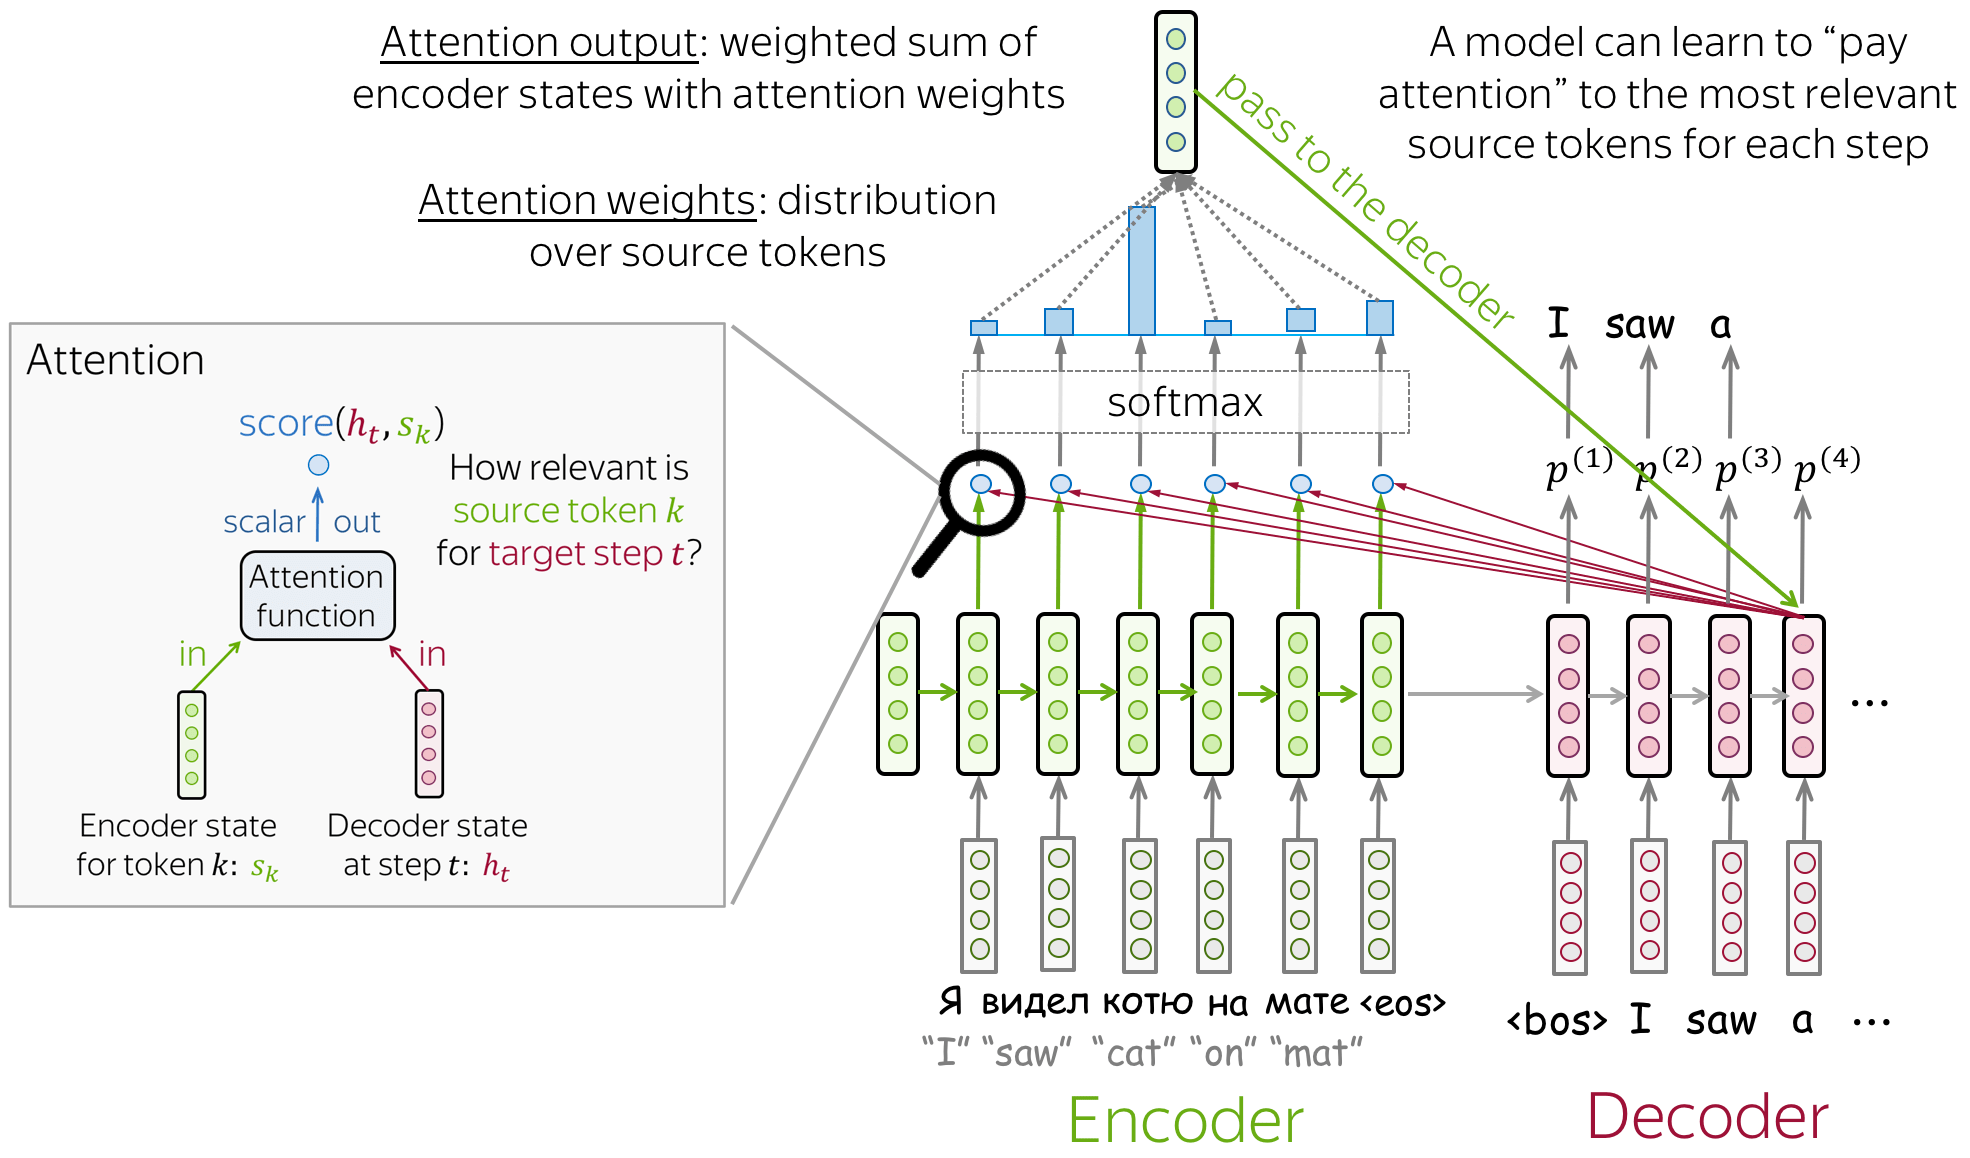
\includegraphics[width=0.8\textwidth]{Images/5.Theoretical_Background/attention_architecture.png}
    \caption{The architecture of the attention mechanism, Source \cite{voita2020nlpCourse}}
    \label{fig:attention_architecture}
\end{figure}

\section{Transformer}
The Transformer architecture is a neural network architecture introduced in the paper titled "Attention is All You Need" by Vaswani et al. in 2017 \cite{attentionIsAllYouNeed}. This is a breakthrough in the field of NLP because, at that time, the RNN models were considered state-of-the-art approaches to handle sequential data, especially in sequence modeling. However, the transformer does not use any of the RNN models, instead, it uses entirely the attention mechanism to capture the dependencies between input and output. The Transformer architecture allows the encoding and decoding at all time steps to be parallelized, so it is faster than the RNN models. The architecture of the Transformer is shown in Figure \ref{fig:transformer_architecture}. To understand the Transformer architecture, firstly, we need to understand the self-attention mechanism.

\begin{figure}[ht]
    \centering
    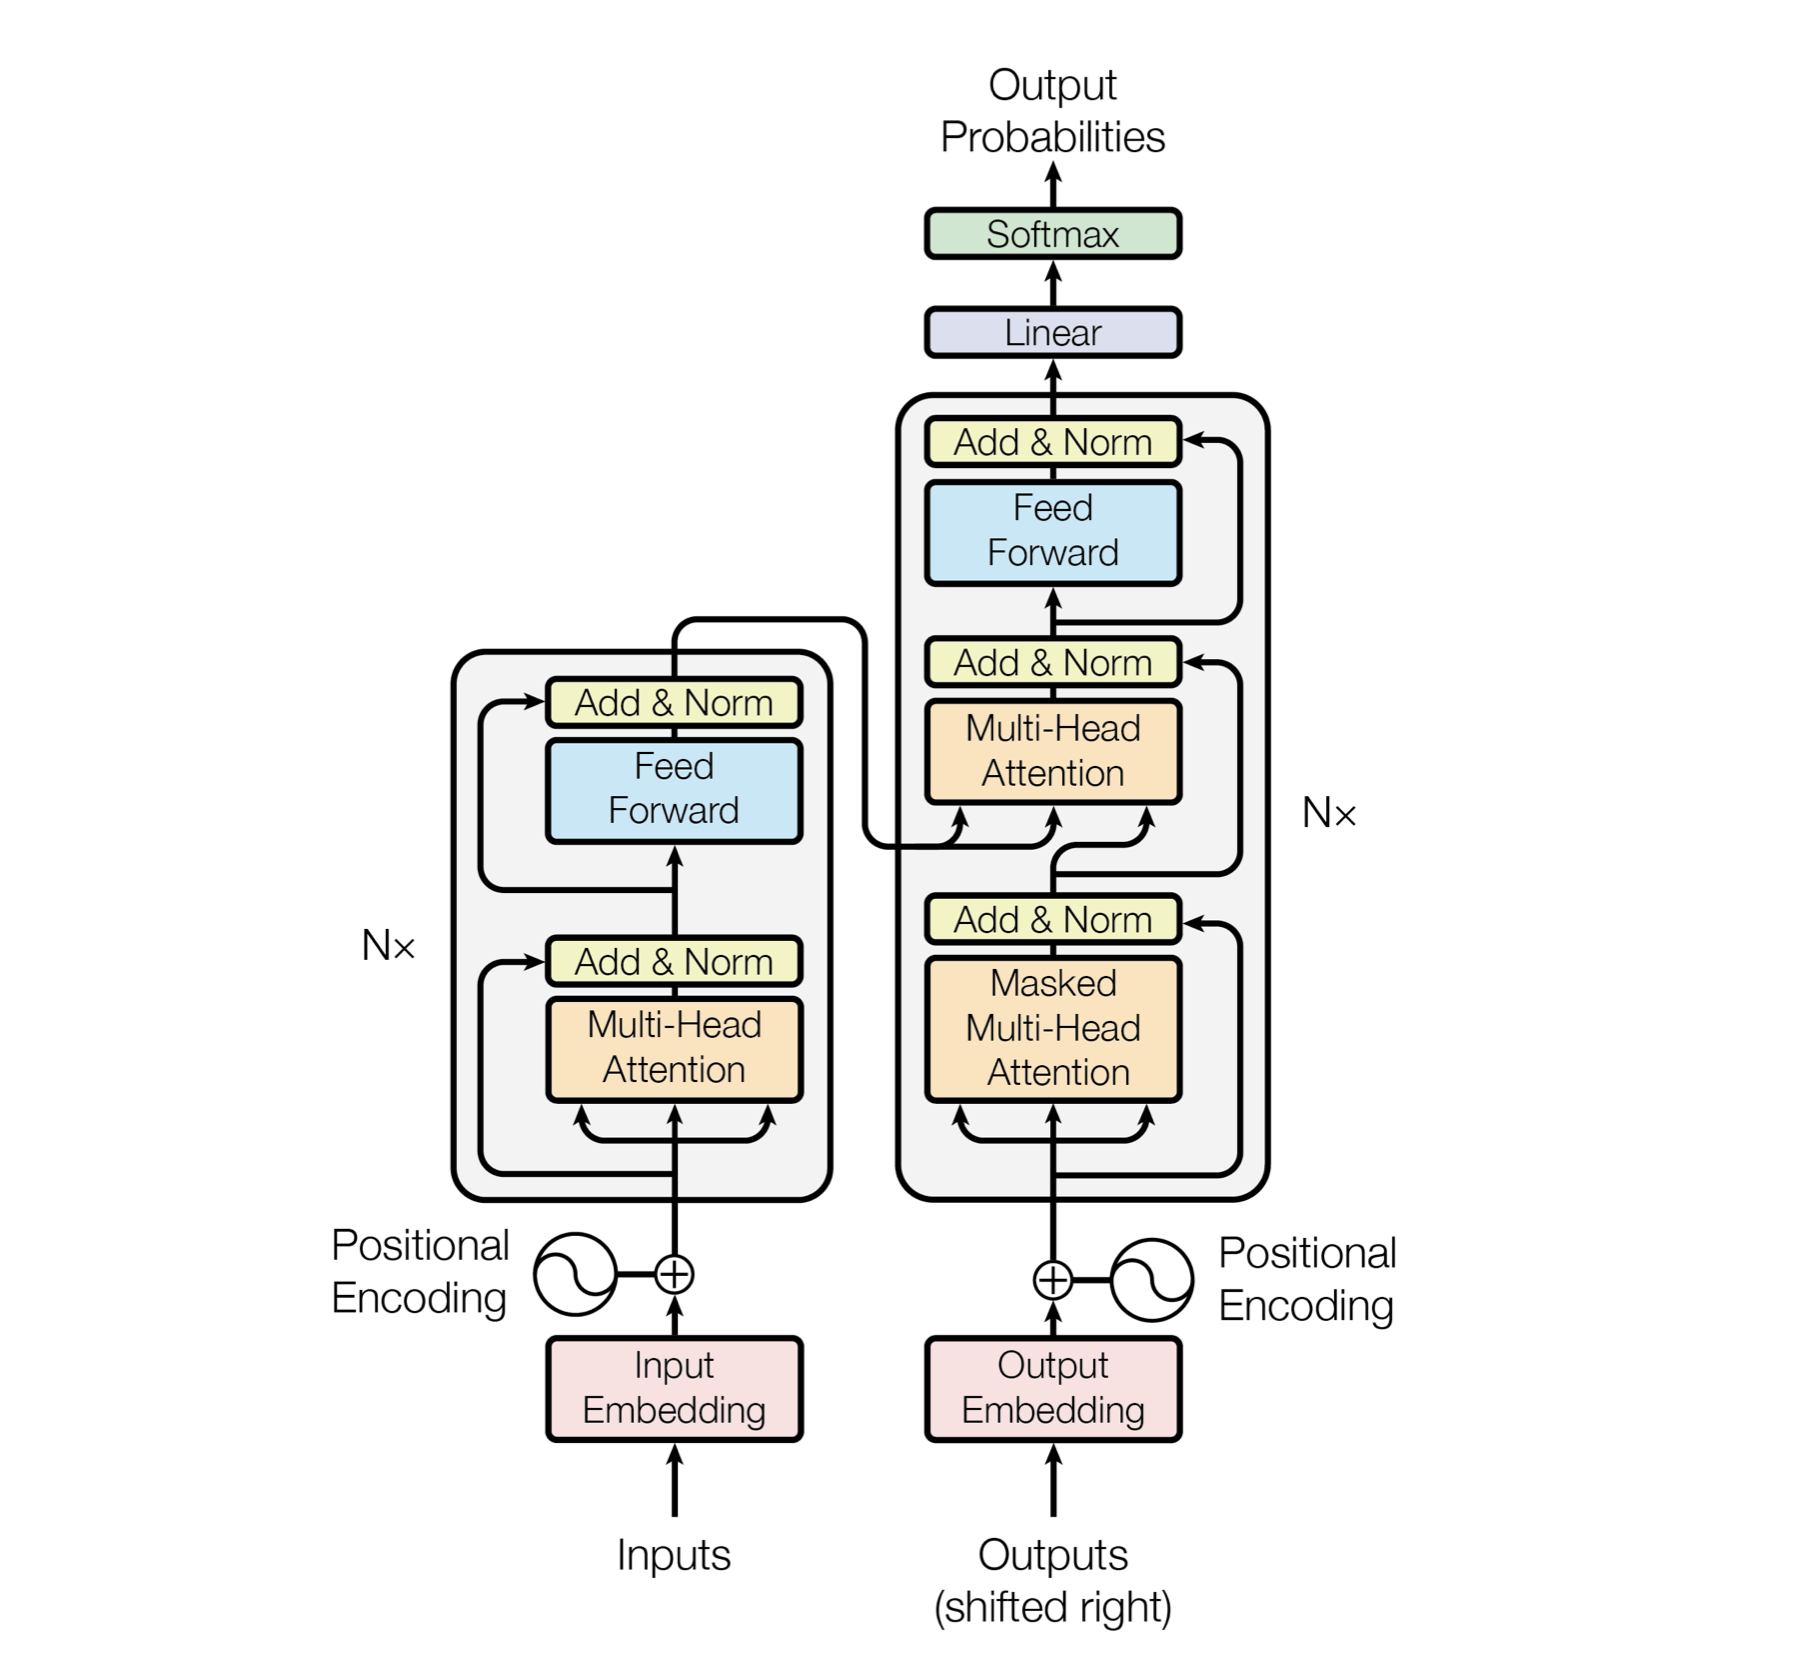
\includegraphics[width=0.8\textwidth]{Images/5.Theoretical_Background/transformer_architecture.png}
    \caption{The architecture of the Transformer proposed in \cite{attentionIsAllYouNeed}}
    \label{fig:transformer_architecture}
\end{figure}

\subsection{Self-Attention mechanism}
Self-Attention mechanism computes the attention score between every pair of words in the input sequence. The attention score shows how relevant is the word $x_j$ for the word $x_i$. The attention score is calculated as follows: 
\begin{enumerate}
    \item Each input token receives three representations: query, key and value.
    \item The attention score between the word $x_i$ and the word $x_j$ is calculated as the dot product between the query of the word $x_i$ and the key of the word $x_j$. The self-attention mechanism also calculates the attention score between the word and itself. 
    \item The weights are calculated by applying the softmax function to the attention scores.
    \item The attention output is calculated as the weighted sum of the value of all words in the input sequence. 
\end{enumerate}

\noindent After applying the self-attention mechanism, we get the output is the same as the input sequence, but the information of each word is updated based on the information of the other words in the input sequence. The self-attention mechanism is shown in Figure \ref{fig:self_attention_mechanism}.

\begin{figure}[ht]
    \centering
    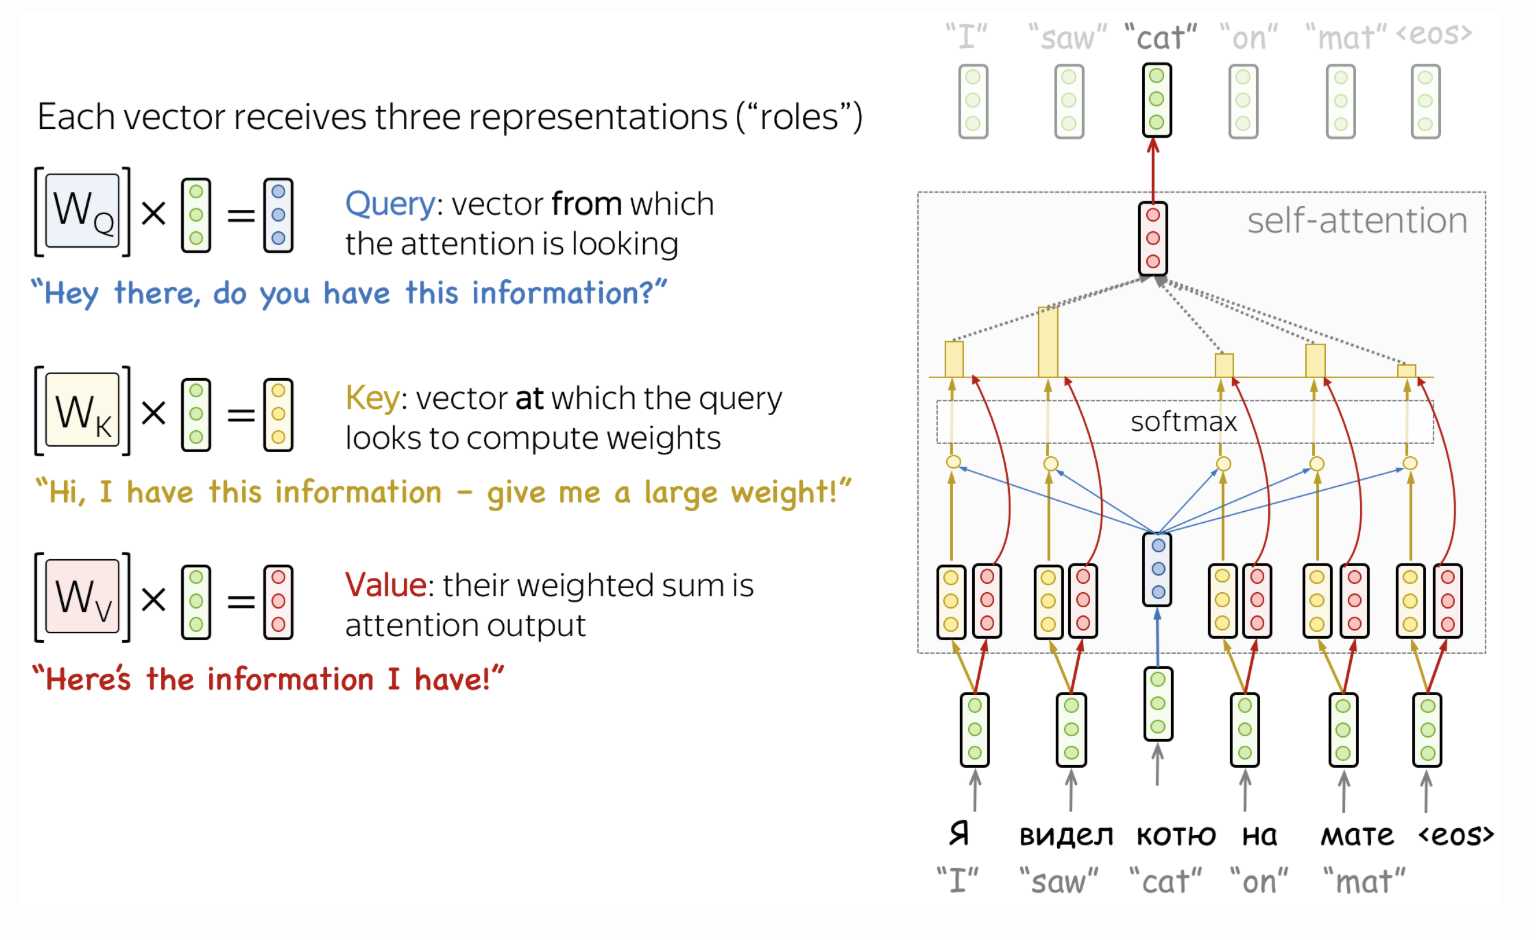
\includegraphics[width=0.8\textwidth]{Images/5.Theoretical_Background/self_attention_mechanism.png}
    \caption{The self-attention mechanism, Source \cite{voita2020nlpCourse}}
    \label{fig:self_attention_mechanism}
\end{figure}

The Self-Attention layers with different parameters can be stacked together to form the Multi-Head Attention layer. The Multi-Head Attention layer allows the model to capture different relationships between the words.

\subsection{Positional Encoding layer}
Because the Transformer does not use any of the RNN models, it cannot capture the position of the words in the input sequence. The Positional Encoding layer is used to solve this problem. The Positional Encoding layer adds the positional information to the input sequence. The Positional Encoding layer is calculated as follows:
\begin{align*}
    PE_{(pos, 2i)} &= sin(pos/10000^{2i/d_{model}}) \\
    PE_{(pos, 2i+1)} &= cos(pos/10000^{2i/d_{model}})
\end{align*}

\noindent Where pos is the position in the text and i is the vector dimension \cite{voita2020nlpCourse}

\subsection{FeedForward layer}
The FeedForward layer is a fully connected layer with a ReLU activation function. The FeedForward layer is used to transform the output of the Multi-Head Attention layer into the output of the Transformer and also process the new information from the Multi-Head Attention layer.

\section{BERT}
BERT (Bidirectional Encoder Representations from Transformers) is a language model proposed by Jacob Devlin et al. in 2018 \cite{bert_jacob}. BERT is a pre-trained language model that is pre-trained on a large corpus of text and can be fine-tuned for many NLP tasks. Besides, BERT is a bidirectional model, so it can capture the context of both sides of the words.


